% Define document class
\documentclass[twocolumn]{aastex631}

% Filler text
\usepackage{blindtext}

% Begin!
\begin{document}

% Title
\title{\showyourwork: a workflow for open source scientific articles}

% Author list
\author[0000-0002-0296-3826]{Rodrigo Luger}

% Abstract with filler text
\begin{abstract}
    \blindtext
\end{abstract}

% Main body with filler text
\section{Introduction}

\begin{figure}[ht!]
    \begin{centering}
        \includegraphics[width=\linewidth]{figures/eccentricity.pdf}
        \caption{
            LEGWORK plot. Figure reproduced from \citet{Wagg2021}.
        }
        \label{fig:eccentricity}
    \end{centering}
\end{figure}

\begin{figure}[ht!]
    \begin{centering}
        \includegraphics[width=\linewidth]{figures/rossbyridge.pdf}
        \caption{
            Rossby ridge. Figure reproduced from David et al. (in prep).
        }
        \label{fig:rossbyridge}
    \end{centering}
\end{figure}

\begin{figure}[ht!]
    \begin{centering}
        \includegraphics[width=\linewidth]{figures/luhman16b.pdf}
        \caption{
            Caption. Figure adapted from \citet{Luger2021}; data originally from \citet{Crossfield2014}.
        }
        \label{fig:luhman16b}
    \end{centering}
\end{figure}

\begin{figure}[ht!]
    \begin{centering}
        \includegraphics[width=\linewidth]{figures/HD118203_transit.pdf}
        \includegraphics[width=\linewidth]{figures/HD118203_corner.pdf}
        \caption{
            The phase-folded transit of HD 118203b in \emph{TESS} (\emph{top}) and the inferred joint posterior distributions over its period, radius, and impact parameter (\emph{bottom}); adapted from the \texttt{exoplanet} documentation \citep{ForemanMackey2021}.
            Both figures were generated from the same \texttt{Python} script in the \texttt{src/figures} directory (linked to in the \texttt{GitHub} icon in the margin). The other margin icon indicates that these figures depend on a dataset (a \texttt{.npz} file containing the posterior samples), which is automatically generated by \showyourwork and uploaded to Zenodo. 
            Users wishing to reproduce the results in this paper can choose whether to re-generate this dataset or download a static version from Zenodo (linked to in the margin).
        }
        \label{fig:HD118203}
    \end{centering}
\end{figure}

\begin{figure}[ht!]
    \begin{centering}
        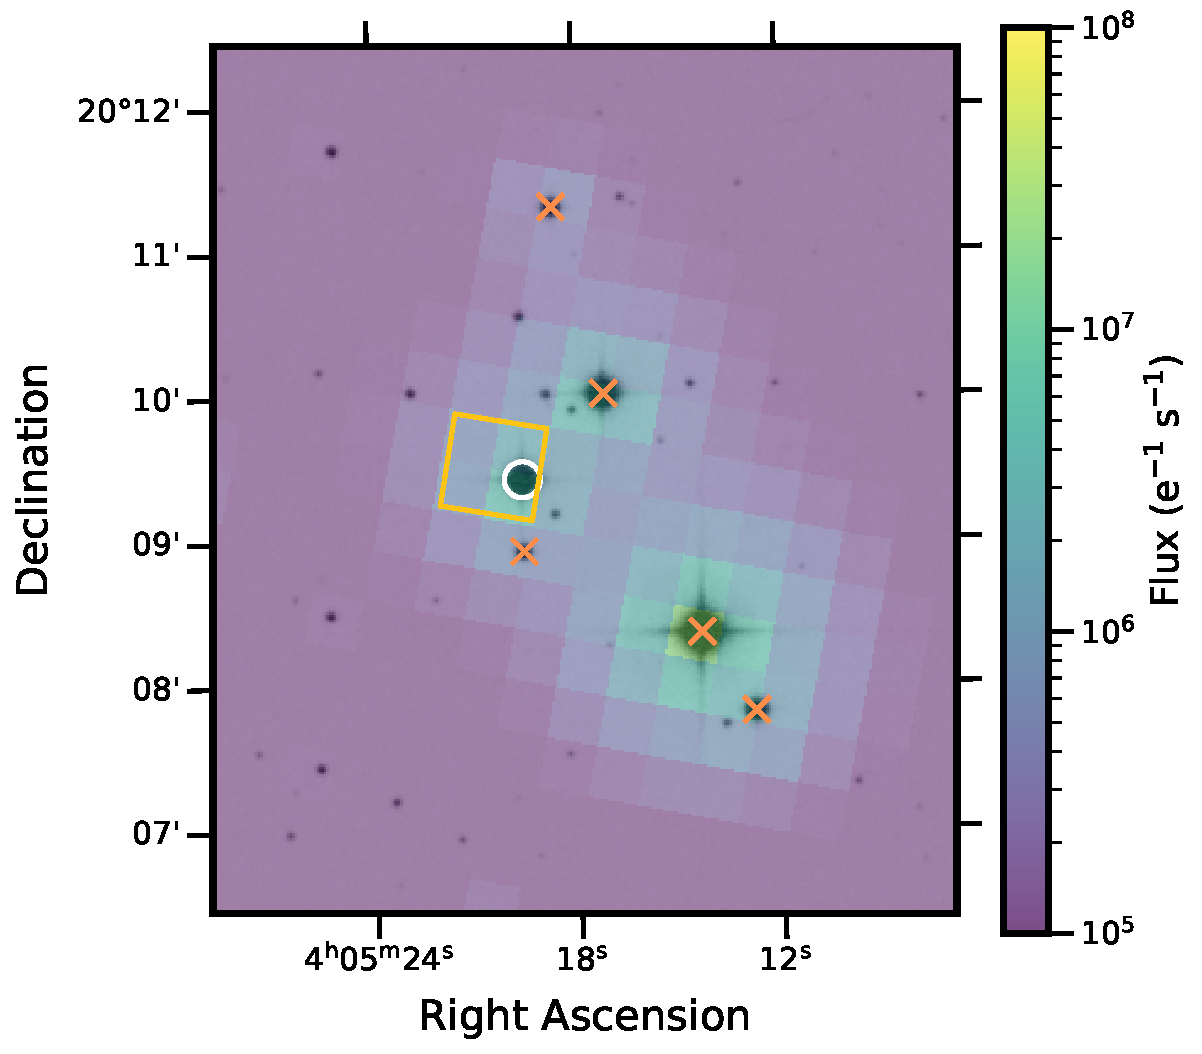
\includegraphics[width=\linewidth]{static/TESSaperture.pdf}
        \caption{
            \emph{TESS} target pixel file (TPF) of V1298 Tau
            overlaid with an r-band sky image from the Digitized Sky Survey (DSS);
            reproduced from Figure 1 in \citet{Feinstein2021}.
            This figure exists as a static PDF, with no associated script to
            generate it.
            We therefore include it in the \texttt{src/static} directory, which tells \showyourwork to not attempt to generate it. 
            By default, margin icons are not added to static figures.
            Here we manually add an icon linking to the original paper using the \texttt{\textbackslash marginicon} command.
        }
        \marginicon{%
            \href{https://ui.adsabs.harvard.edu/abs/2021arXiv211108660F}{\color{sywBlue}\faNewspaper[regular]}
        }
        \label{fig:eclipse}
    \end{centering}
\end{figure}

\begin{figure*}[ht!]
    \begin{centering}
        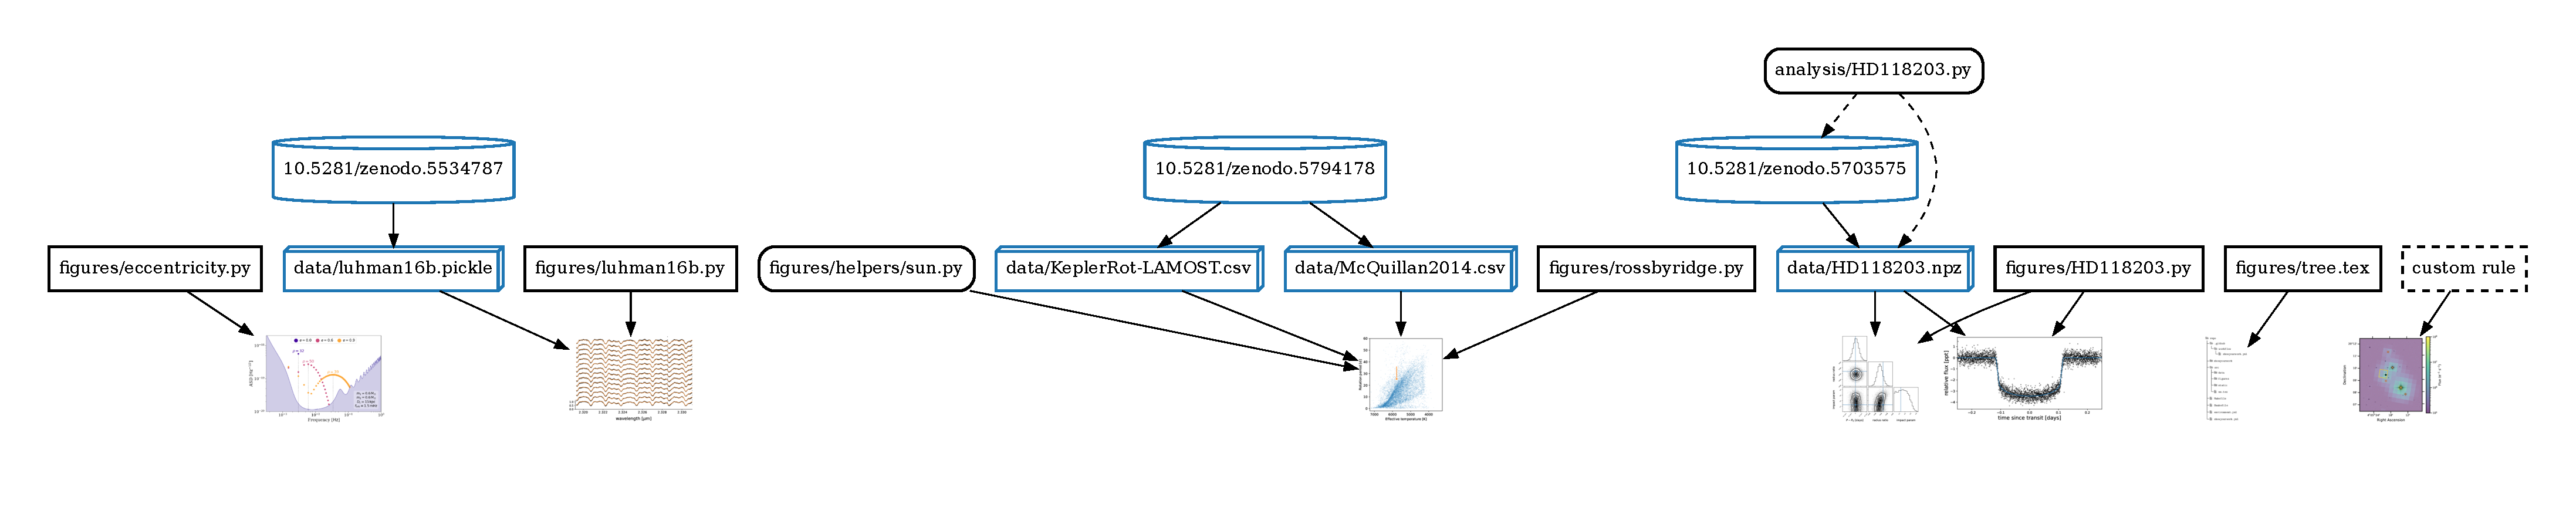
\includegraphics[width=\linewidth]{figures/dag.pdf}
        \caption{
            A directed acyclic graph (DAG) showing the build process for each of the (other) figures in this article. 
        }
        \label{fig*:dag}
    \end{centering}
\end{figure*}

\bibliography{bib}

\end{document}
